We evaluate SPORES to answer three research questions about our
approach of relational equality saturation: 
\begin{itemize}
    \item \textbf{Section~\ref{relcomp}}: can SPORES derive hand-coded
      rewrite rules for sum-product optimization?
    \item \textbf{Section~\ref{perf}}: can SPORES find optimizations that
      lead to greater performance improvement than hand-coded rewrites and
      heuristics? 
      \item \textbf{Section~\ref{overhead}}: does SPORES induce compilation overhead afforded by its performance gain?  
\end{itemize}

We ran experiments on a single node with Intel E74890 v2 @ 2.80GHz with hyper-threading, 
1008 GB RAM, 8TB
disk, and Ubuntu 16.04.6. We used OpenJDK 1.8.0, Apache Hadoop 2.7.3, and Apache
Spark 2.4.4. Spark was configured to run locally with 6 executors, 8
cores/executor, 50GB driver memory, and 100GB executor memory. Our baselines are
from Apache SystemML 1.2.0. All datasets have been synthetically generated to
evaluate a range of scenarios, where we used algorithm specific data generators
from SystemML's benchmark suite.

\subsection{Completeness of Relational Rules} \label{relcomp}
% \begin{figure}
% \begin{enumerate}
%   \item $sum(A+B) = sum(A)+sum(B)$
%   \item $sum(X^T) = sum(X)$
%   \item $sum(sum_{row}(X)) = sum(X)$,  $sum_{col}$ similar
%   \item $(UV)^T = V^TU^T$, $(U*V)^T=U^T*V^T$
%   \item $(A+B)^T=A^T + B^T$, $(X^T)^T=X$
%   \item $(X*Y)*Z = X*(Y*Z)$, $X*Y = Y*X$
%   \item $A * X + b * X =  (A+b)*X$
%   \item $a * UV = (a*U) V$
% \end{enumerate}
% \caption{LA equality rules $R_{LA}$ for comparison. \textcolor{red}{TODO fix caption}}
% \label{RLA}
% \end{figure}

\begin{figure}
    \centering
    \begin{tabular}{|l|c|l|}
    \hline
     Method Name & \# & Example Rewrite \\
     \hline
     
\verb|UnnecessaryOuterProduct| & 3 & \verb|X*(Y%*%1) ->| \verb| X*Y, if Y col vector |\\

\verb|ColwiseAgg| & 3 & \verb|colsums(X) -> sum(X) or X, if col/row vector |\\

\verb|RowwiseAgg| & 3 & \verb|rowsums(X) -> sum(X) or X, if row/col vector |\\

\verb|ColSumsMVMult| & 1 & \verb|colSums(X*Y) -> t(Y) %*% X, if Y col vector |\\

\verb|RowSumsMVMult| & 1 & \verb|rowSums(X*Y) -> X %*% t(Y), if Y row vector |\\

\verb|UnnecessaryAggregate| & 9 & \verb|sum(X) -> as.scalar(X), if 1x1 dims |\\
\verb|EmptyAgg| & 3 & \verb|sum(X) -> 0, if nnz(X)==0 |\\
\verb|EmptyReorgOp| & 5 & \verb|t(X) -> matrix(0, ncol(X), nrow(X)) if nnz(X)==0|\\
\verb|EmptyMMult| & 1 & \verb|X%*%Y -> matrix(0,...), if nnz(Y)==0|\\
\verb|IdentityRepMatrixMult| & 1 & \verb|X%*%y -> X if y matrix(1,1,1) |\\
\verb|ScalarMatrixMult| & 2 & \verb|X%*%y -> X*as.scalar(y), if y is a 1-1 matrix |\\
\verb|pushdownSumOnAdd| & 2 & \verb|sum(A+B) -> sum(A)+sum(B) if dims(A)==dims(B) |\\

\verb|DotProductSum| & 2 & \verb|sum(v^2) -> t(v)%*%v if ncol(v)==1 |\\
\verb|reorderMinusMatrixMult| & 2 & \verb|(-t(X))%*%y -> -(t(X)%*%y) |\\

\verb|SumMatrixMult| & 3 & \verb|sum(A%*%B) -> sum(t(colSums(A))*rowSums(B)) |\\
\verb|EmptyBinaryOperation| & 3 & \verb|X*Y -> matrix(0,nrow(X),ncol(X)) / X+Y->X / X-Y->X |\\
\verb|ScalarMVBinaryOperation| & 1 & \verb|X*y -> X*as.scalar(y), if y is a 1-1 matrix |\\
\verb|UnnecessaryBinaryOperation| & 6 & \verb|X*1 -> X (after rm unnecessary vectorize) |\\
\verb|BinaryToUnaryOperation| & 3 & \verb|X*X -> X^2, X+X -> X*2, (X>0)-(X<0) -> sign(X) |\\
\verb|MatrixMultScalarAdd| & 2 & \verb|eps+U%*%t(V) -> U%*%t(V)+eps|\\
\verb|DistributiveBinaryOperation| & 4 & \verb|(X-Y*X) -> (1-Y)*X |\\
\verb|BushyBinaryOperation| & 3 & \verb|(X*(Y*(Z%*%v))) -> (X*Y)*(Z%*%v) |\\
\verb|UnaryAggReorgOperation| & 3 & \verb|sum(t(X)) -> sum(X) |\\
\verb|UnnecessaryAggregates| & 8 & \verb|sum(rowSums(X)) -> sum(X) |\\
\verb|BinaryMatrixScalarOperation| & 3 & \verb|as.scalar(X*s) -> as.scalar(X)*s |\\

\verb|pushdownUnaryAggTransposeOp| & 2 & \verb|colSums(t(X)) -> t(rowSums(X)) |\\
\verb|pushdownCSETransposeScalarOp| & 1 & \verb|a=t(X), b=t(X^2) -> a=t(X), b=t(X)^2 for CSE t(X) |\\

\verb|pushdownSumBinaryMult| & 2 & \verb|sum(lamda*X) -> lamda*sum(X) if lamdba is scalar|\\
\verb|UnnecessaryReorgOperation| & 2 & \verb|t(t(X))->X potentially introduced by other rewrites |\\
\verb|TransposeAggBinBinaryChains| & 2 & \verb|t(t(A)%*%t(B)+C) -> B%*%A+t(C) |\\
\verb|UnnecessaryMinus| & 1 & \verb|-(-X)->X potentially introduced by other rewrites |\\
\hline
\end{tabular}{}
    \caption{Sum-product rewrites in SystemML. The first column lists the name for each rewrite method. Each 
    method implements a number of rewrite patterns, and the second column shows how many. The last column shows an example rewrite for each method. Following SystemML's notation, scalars are in lower-case and matrices/vectors in upper-case. \texttt{\%*\%} is matrix multiply,  \texttt{t()} is transpose, and \texttt{nnz(X)} is the number of non-zeroes in $X$. 
    Equality saturation derives rewrites form all 31 methods (84 patterns) with relational  rules. }
    \label{rewritecomplete}
\end{figure}{}

Theoretically, our first hypothesis is validated by the fact that our relational
equality rules are complete w.r.t. linear algebra semantics. To test completeness in
practice\footnote{\textit{``I have only proved it correct, not tried it''} --
  Donald Knuth}, our first set of experiments check if SPORES
can derive the hand-coded sum product rewrite rules in SystemML. To do this, we
input the left hand side of each rule into SPORES, perform equality
saturation, then check if the rule's right hand side is present in the saturated
graph. The optimizer is able to derive
all 84 sum-product rewrite rules in SystemML using relational equality rules. 
See Figure~\ref{rewritecomplete} for a list of these rewrites. 
We believe replacing the 84 ad-hoc
rules with our translation rules $R_{LR}$ and equality rules $R_{EQ}$ would greatly
simplify SystemML's codebase. Together with equality saturation, our relational
rules can also lead to better performance, as we demonstrate in the next set of
 experiments.

% We then replace the RA equalities with the usual
% linear algebra equalities listed in Figure~\ref{RLA} and perform the same test.
% This time, the optimizer can only derive 33 out of 59 rules.
% TODO get number

% While we argue the experiment shows the benefit of RA rules over LA rules, one
% may wonder if we over-constrain the LA rules; perhaps 
% by adding a few additional rules, the LA rules can become complete as well. To
% this we answer that our RA rules can be viewed as an enhanced version of LA
% rules. While there may be other alternatives, we have shown our rules to be apt
% both in theory and in practice. From a different angle, the rules in
% Figure~\ref{rewritecomplete} from SystemML can also be regarded as an enhanced
% version of LA equalities. However, it is incomplete because it cannot derive 
% our example optimization of $sum((X-UV^T)^2)$. Practically, our RA rules are both more
% principled and simpler than the hand-coded rules, so adopting the former can
% simplify the codebase and alleviate maintenance burden. Together with equality saturation, our RA
% rules can also lead to better performance, as we demonstrate in the next set of
% experiments.

% TODO runtime evaluation 
\subsection{Run Time Measurement} \label{perf}

\begin{figure*}
    \centering  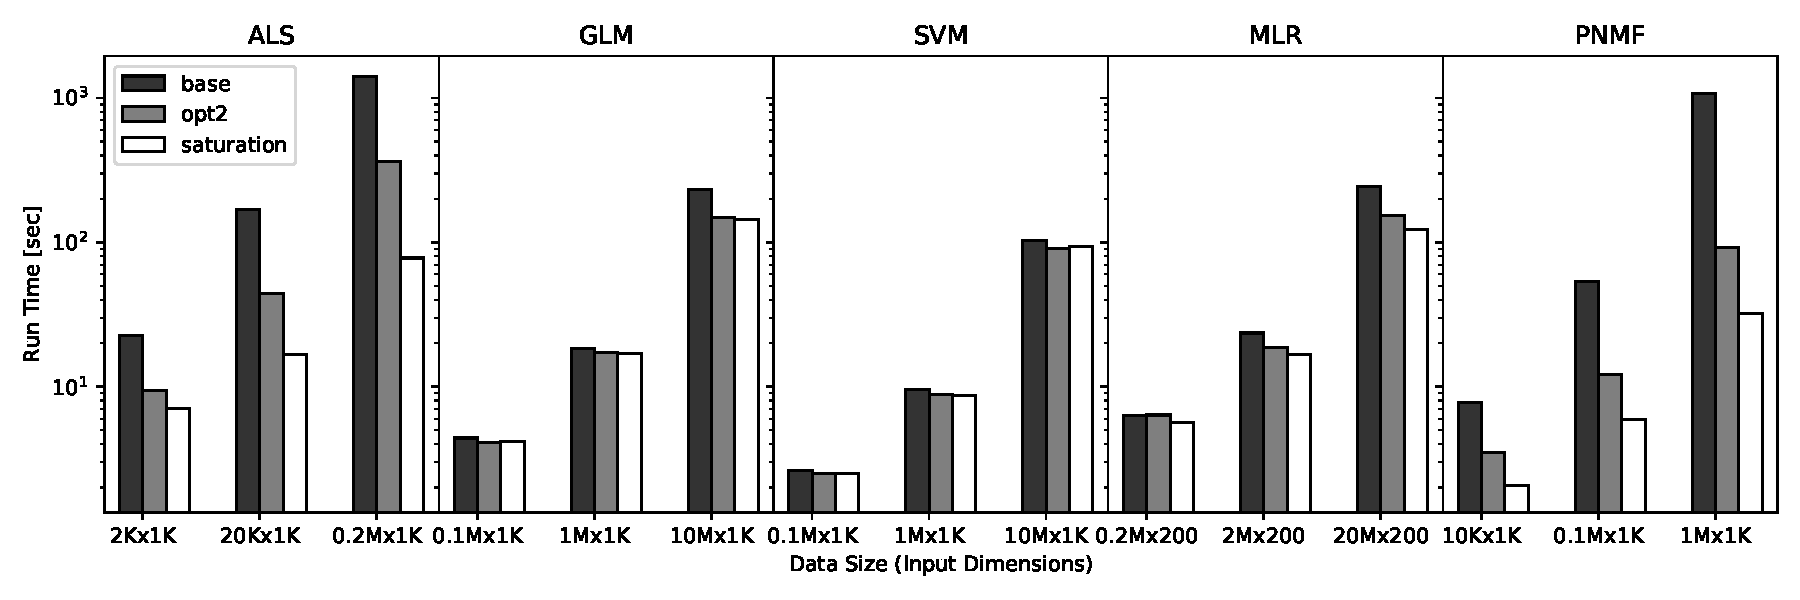
\includegraphics[width=\textwidth]{runtime.pdf}
    \caption{Run time of programs compiled by different optimizers. }
    \label{eval}
\end{figure*}
% \textcolor{red}{TODO: fix caption}

\begin{figure*}
    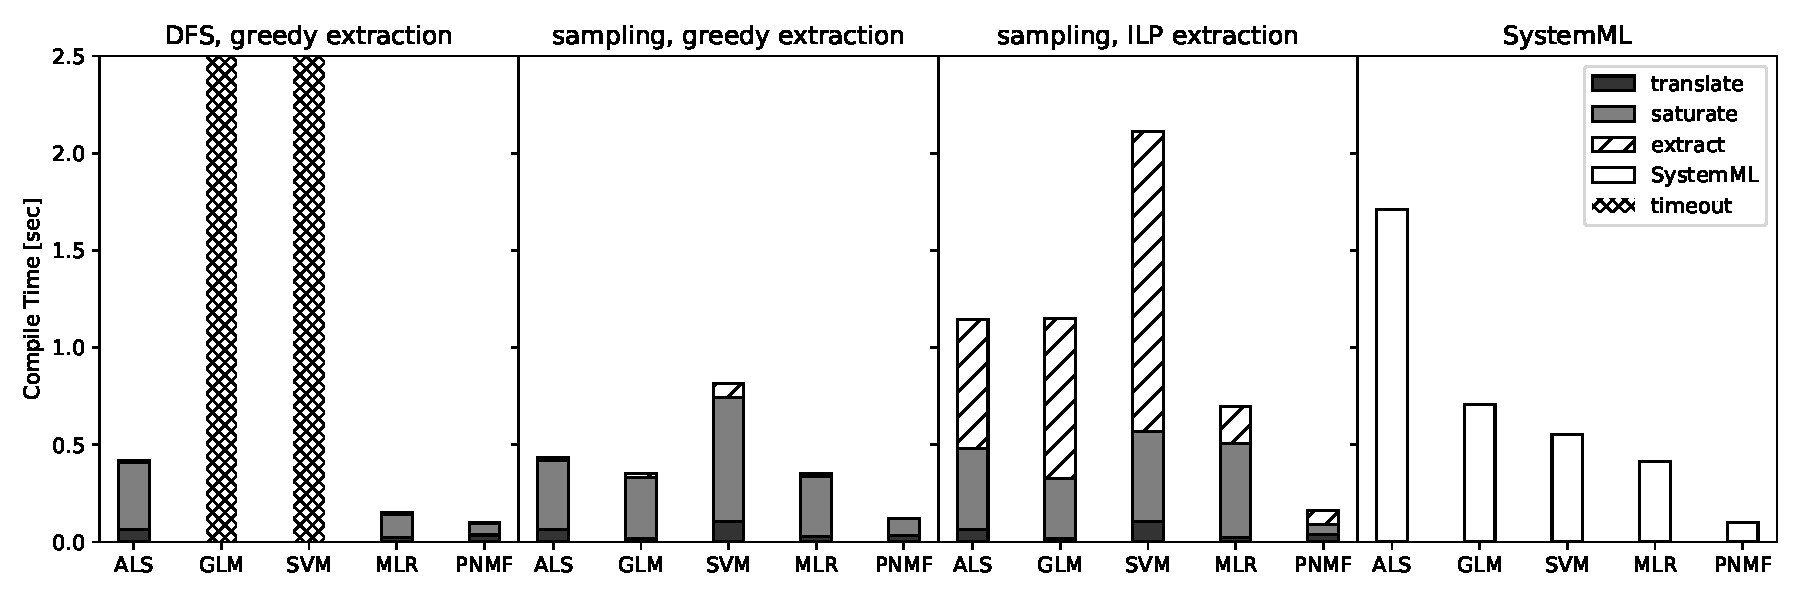
\includegraphics[width=\textwidth]{compiletime.pdf}
    \caption{Compile time breakdown for different saturation and extraction
      strategies. Depth-first saturation reaches the 2.5s timeout compiling GLM and SVM. }
    \label{compile}
\end{figure*}{}
% {TODO: caption this}
We compare SPORES against SystemML's native optimizations for their
performance impact. In particular, we run SystemML with optimization level 2 (\texttt{opt2}),
which is its default and includes all advanced rewrites like constant folding
and common subexpression elimination. We additionally enable SystemML's native
sum-product rewrites and operator fusion. 
For baseline (\texttt{base}) we use level 1 optimization from SystemML, since level 0 (no optimization)
timeouts on almost all input sizes. \texttt{base} includes no advanced rewrites, 
sum-product optimization or operator fusion; it only performs local optimizations
with basic pattern-matching. 
We compile and execute 5 real-world
algorithms under 3 configurations:
\begin{enumerate*}
    \item SystemML without optimization,
    \item SystemML with optimization configured as above, and
    \item our equality saturation optimizer.
\end{enumerate*}{}
 The algorithms include Generalized Linear Model (GLM), Multinomial
 Logistic Regression (MLR), Support Vector Machine (SVM), Poisson
 Nonnegative Matrix Factorization (PNMF), and Alternating Least Square
 Factorization (ALS). We take the implementation of these algorithms from
 SystemML's performance benchmark suite.

Figure~\ref{eval} shows the performance improvement for each optimization
setting. Overall, equality saturation is competitive with the hand-coded rules
in SystemML: for GLM and SVM, saturation discovers the same
optimizations that improve performance as SystemML does. For ALS, MLR and PNMF,
saturation found new optimizations that lead to speedups from 1.2X to 5X
as compared to SystemML. We analyze each benchmark in
detail in the following paragraphs.

% \begin{figure}[t]
% \begin{lstlisting}[language=R]
% H=H*(t(W)%*%(X/(W%*%H+eps)))/t(colSums(W))
% W=W*((X/(W%*%H+eps))%*%t(H))/t(rowSums(H))
% obj=sum(W%*%H)-sum(X*log(W%*%H+eps))
% \end{lstlisting}
%     \caption{PNMF main loop. $X$ is a sparse matrix, $W$ and $H$ are low-rank matrices, and
%       $eps$ is a scalar.}
%     \label{pnmf}
% \end{figure}
% \begin{figure}[t]
% \begin{lstlisting}[language=R]
% Q=P[,1:K] * (X %*% ssX_V)
% HV=t(X)%*%(Q - P[,1:K]
%       *(rowSums(Q)%*%matrix(1,1,K)))
% \end{lstlisting}
%     \caption{Part of MLogReg main loop. $X$ and $ssX\_V$ are matrices. In our experiment $K=1$ so
%       $P[,1:K]$ and $Q$ are column vectors, and $matrix(1,1,K)$ is a 1x1
%       matrix holding the value $1$. }
%     \label{mlogreg}
% \end{figure}



% TODO no section 
% \subsection{Rewrite Details} \label{optdetails}

For \textbf{ALS}, SPORES leads to up to 5X speedup beyond SystemML's
optimizations using our relational rules. Investigating the optimized code
reveals the speedup comes from a rather simple optimization: SPORES expands
$(UV^T - X)V$ to $UV^TV-XV$ to exploit the sparsity in $X$. Before the optimization,
all three operations (2 matrix multiply and 1 minus) 
in the expression create dense intermediates because $U$
and $V$ are dense. After the optimization, $XV$ can be computed efficiently thanks to
the sparsity in $X$. $UV^TV$ can be computed in one go without intermediates, taking advantage of
SystemML's \texttt{mmchain} operator for matrix multiply chains. Although the
optimization is straightforward, it is counter-intuitive because one expects
computing $A(B + C)$ is more efficient than $AB + AC$ if one does not consider
sparsity. For the same reason, SystemML simply does not consider distributing
the multiplication and misses the optimization.

For \textbf{PNMF}, the speedup of up to 3X using RA rules attributes to rewriting $sum(WH)$
to $sum_{col}(W) \cdot sum_{row}(H)$ which avoids materializing a dense
intermediate $WH$. Interestingly, SystemML includes this rewrite rule but did
not apply it during optimization. In fact, SystemML only applies the rule when
$WH$ does not appear elsewhere, in order to preserve common subexpression.
However, although $WH$ is shared by another expression in PNMF, the other
expression can also be optimized away by another rule. Because both rules uses heuristics to favor sharing CSE, neither fires. 
This precisely
demonstrates the limitation of heuristics. 

For \textbf{MLR}, the important optimization\footnote{Simplified here for
  presentation. In the source code $P$ and $X$ are not variables but consist of
  subexpressions. } by saturation is $P * X - P * sum_{row}(P) * X$ to
$P*(1-P)*X$, where $P$ is a column vector. This takes advantage of the
\texttt{sprop} fused operator in SystemML to compute $P*(1-P)$, therefore
allocating only one intermediate. Note that the optimization factors out $P$, which
is the exact opposite to the optimization in ALS that distributes multiply. Naive
rewrite rules would have to choose between the two directions, or resort to
heuristics to decide when to pick which. 

% TODO check dimensions
% \begin{figure}[t]
% \begin{lstlisting}[language=R]
% out=1-Y*(Xw+step_sz*Xd);
% sv=(out>0);
% out=out*sv;
% g=wd+step_sz*dd-sum(out*Y*Xd); 
% h=dd+sum(Xd*sv*Xd);
% step_sz = step_sz - g/h;
% \end{lstlisting}
%     \caption{Part of L2SVM main loop. }
%     \label{l2svm}
% \end{figure}
% \begin{figure}[t]
% \begin{lstlisting}[language=R]
% t_gp=1.0/(1.0+abs(flt)*0.231641888)
% pt_gp = t_gp * ( 0.254829592 
%       + t_gp * (-0.284496736 
%       + t_gp * ( 1.421413741 
%       + t_gp * (-1.453152027 
%       + t_gp *   1.061405429))));
% \end{lstlisting}
%     \caption[gauss error function]{
%     Part of GLM main loop (approximates the Gauss error function~\cite{abramowitz+stegun}). $t\_gp$ is a matrix.}
%     \label{glm}
% \end{figure}

For \textbf{SVM} and \textbf{GLM}, equality saturation finds the same optimizations as
SystemML does, leading to speedup mainly due to operator fusion. Upon
inspection, we could not identify better optimizations for \textbf{SVM}. For
\textbf{GLM}, however, we discovered a manual optimization that should improve
performance in theory, but did not have an effect in practice since SystemML
cannot accurately estimate sparsity to inform execution. 

\subsection{Compilation Overhead} \label{overhead}
\begin{figure*}
    \centering  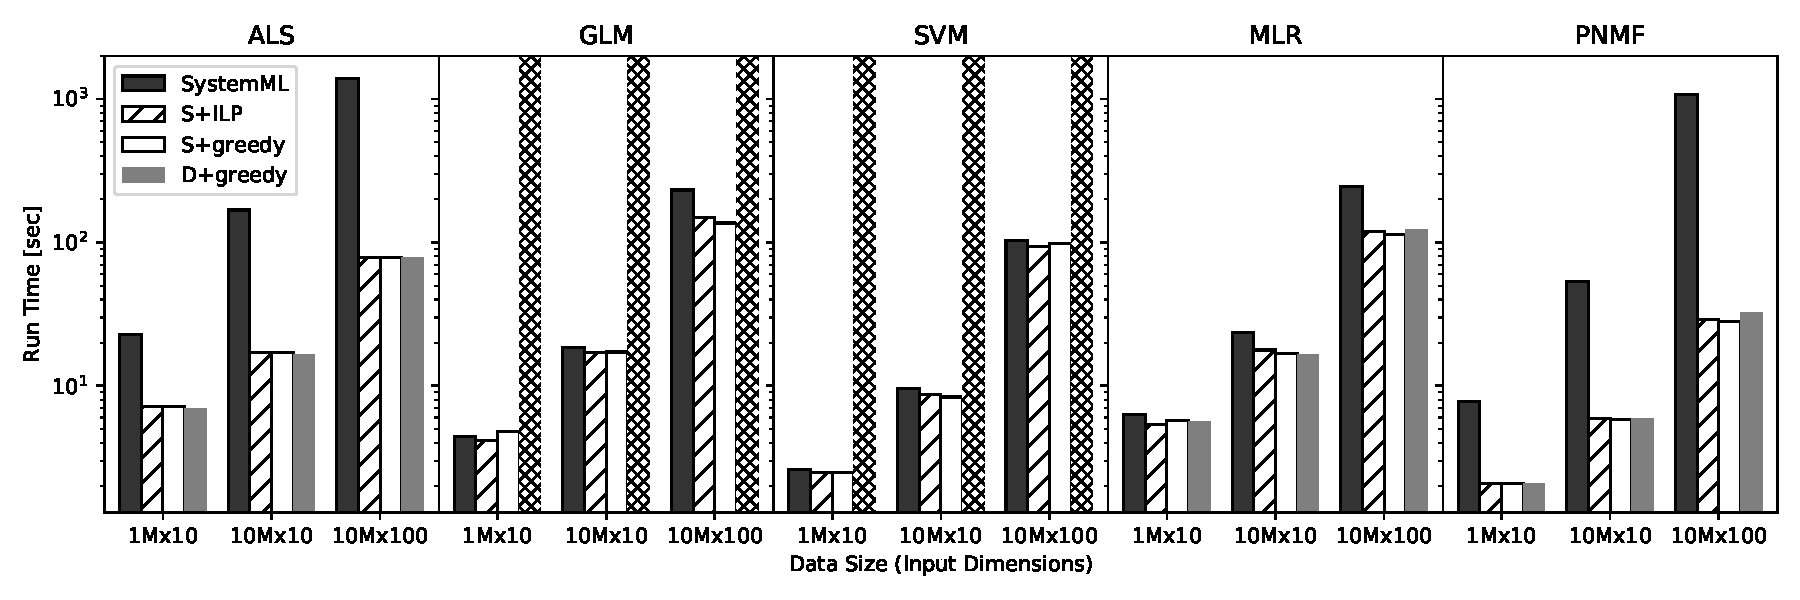
\includegraphics[width=\textwidth]{strategy.pdf}
    \caption{Performance impact of different saturation and extraction
      strategies. S is saturation with sampling, and D is depth-first saturation. Depth-first saturation runs into timeout compiling GLM and SVM. }
    \label{sampleeval}
\end{figure*}
% TODO find number \textcolor{red}{TODO fix caption}}
In our initial experiments, SPORES induces nontrivial compilation
overhead compared to SystemML's native rule-based rewrites. Figure~\ref{compile}
 (sampling, ILP extraction) shows the compile time breakdown for each benchmark, and the majority of time is
spent in the ILP solver. We therefore experiment with a greedy algorithm during
extraction to see if we can trade off guarantees of optimality for a shorter
compile time. This algorithm traverses the saturated graph bottom-up, picking
the cheapest operator in each class at every level. Figure~\ref{sampleeval}
shows the performance impact of greedy extraction, and Figure~\ref{compile} (sampling, greedy extraction)
shows the compile time with it. Greedy extraction significantly reduces compile
time without sacrificing \textit{any} performance gain! This is not surprising
in light of the optimizations we discussed in Section~\ref{perf}: all of
these optimizations improve performance regardless of common
subexpressions, so they are selected by both the ILP-based and the greedy
extractor.

We also compare saturation with sampling against depth-first saturation in terms of
performance impact and compile time. Recall the depth-first saturation strategy
applies all matches per rule per iteration. As Figure~\ref{compile} shows,
sampling is slightly slower for ALS, MLR and PNMF, but resolves the timeout for 
GLM and SVM. This is because sampling takes longer to converge when full
saturation is possible, and otherwise prevents the graph from blowing up before
reaching the iteration limit.
Indeed, saturation converges for ALS, MLR and PNMF, which means SPORES
can guarantee the optimality of its result under the given cost model. Saturation
does not not converge before reaching the iteration limit for GLM and SVM because
of deeply nested $*$ and $+$ in the programs. 
Convergence
may come as a surprise despite E-Graph's compaction -- expansive rules like
associativity and commutativity commonly apply in practice. However, the expression
DAGs we encounter are often small (no more than 15 operators), and large DAGs
are cut into small pieces by optimization barriers like uninterpreted functions. 

Figure~\ref{compile} compares the overall DAG compilation overhead of SystemML
against SPORES with different extraction strategies.
Note that the overhead of SystemML also includes optimizations unrelated to sum-product rewrites that are difficult to disentangle, therefore it only gives a sense of the base compilation time and does not serve as head-to-head comparison against SPORES. 
Although SPORES induces significant compilation overhead in light of SystemML's total DAG compilation time, the overhead is afforded by
its performance gain. As we did not focus our efforts on
reducing compile time, we believe there is plenty room for improvement, for
example organizing rewrite rules to speed up saturation.